%FOR PDFLATEX USE ONLY
\documentclass[a4paper,12pt]{article}

\usepackage{amssymb,amsmath} %math symbols

\usepackage[margin=2cm]{geometry} %paper geometry

\usepackage[utf8]{inputenc} %allows unicode (including russian) source file
\usepackage[russian]{babel} %docment in russian-style
\usepackage[utf8]{inputenc}
%\usepackage[unicode]{hyperref} %links inside of the text
\usepackage[pdftex]{graphicx} %includegraphics pictures
\usepackage{cmlgc} %bold text

\usepackage{array} %arrays

%\usepackage{wrapfig}
%\usepackage{array}
%\usepackage{lipsum}
%\usepackage{esvect}
%\usepackage{hyperref}

\usepackage{subfig}
%\usepackage{calc}
%\usepackage{pgfplots,tikz,circuitikz}
%\usepackage{tkz-euclide}
\usepackage{booktabs}
\usepackage{multirow}

\usepackage{wrapfig}

\begin{document}

\begin{center}
  \LARGE{Работа 4.3.4}\\[0.2cm]
  \LARGE{Метод преобразования Фурье в оптике}\\[0.2cm]
  \large{Малиновский Владимир}\\[0.2cm]
  \normalsize{\texttt{galqiwi@galqiwi.ru}}
\end{center}

\textbf{Цель работы}: Пронаблюдать дифракционные картины и происследовать их с точки зрения разложения разложения в ряд Фурье порождающего шаблона.

\textbf{В работе используются}: Гелий-неоновый лазер, кассета с набором сеток разного периода, щель с микрометрическим винтом, линзы, экран, линейка.

\section*{Теория}
Анализ сложного волнового поля во многих случаях целесообразно проводить, разлагая его на простейшие составляющие, например, представляя его в виде разложения по плоским волнам. При этом оказывается, что если мы рассматриваем поле, полученное после прохождения плоской монохроматической волны через предмет или транспарант (изображение предмета на фотоплёнке или стеклянной пластинке) с функцией пропускания $t(x)$, то разложение по плоским волнам соответствует преобразованию Фурье от этой функции. Если за предметом поставить линзу, то каждая плоская волна сфокусируется в свою точку в задней фокальной плоскости линзы. Таким образом, картина, наблюдаемая в фокальной плоскости линзы, даёт нам представление о спектре плоских волн падающего на линзу волнового поля. Поэтому можно утверждать, что с помощью линзы в оптике осуществляется пространственное преобразование Фурье.

\section*{Определение ширины щели с помощью линзы}
\subsection*{1-3}
Включим лазер и соберем установку, установив вплотную к лазеру тубус с щелью и получив изображение щели на экране с помощью короткофокусной линзы.

\begin{center}
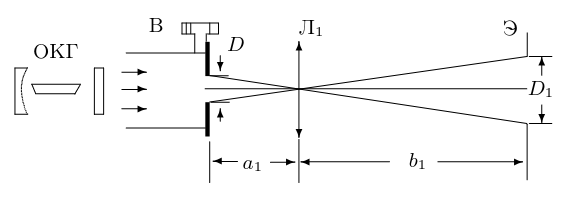
\includegraphics[width=0.95\textwidth]{1.png}
\end{center}

\subsection*{4}
Определим начало отсчета щели по ее открытию. Получим значение $D_0 = (0.140\pm0.005)\,\text{мм}$

\subsection*{5}
Измерим ширину размера изображения $D_1$ в зависимости от ширины щели $D$. Изменение ширины щели будем вести в сторону увеличения, чтобы исключить влияние люфта.

\begin{center}
\begin{tabular}{|c|c|c|}\hline
$D_{\text{raw}}\text{, мкм}$&$D\text{, мкм}$&$D_1\text{, мм}$\\\hline
$140$&$0$&$0.0$\\\hline
$200$&$60$&$4.0$\\\hline
$250$&$110$&$7.0$\\\hline
$300$&$160$&$10.0$\\\hline
$350$&$210$&$12.0$\\\hline
$400$&$260$&$15.0$\\\hline
$450$&$310$&$17.0$\\\hline
$500$&$360$&$20.0$\\\hline
$550$&$410$&$23.0$\\\hline
$600$&$460$&$25.0$\\\hline
$650$&$510$&$30.0$\\\hline
\end{tabular}\\~\\
$\Delta D_{\text{raw}}=5\,\text{мкм}, \Delta D=7\,\text{мкм}, \Delta D_1=0.5\,\text{мм}$
\end{center}


\begin{center}
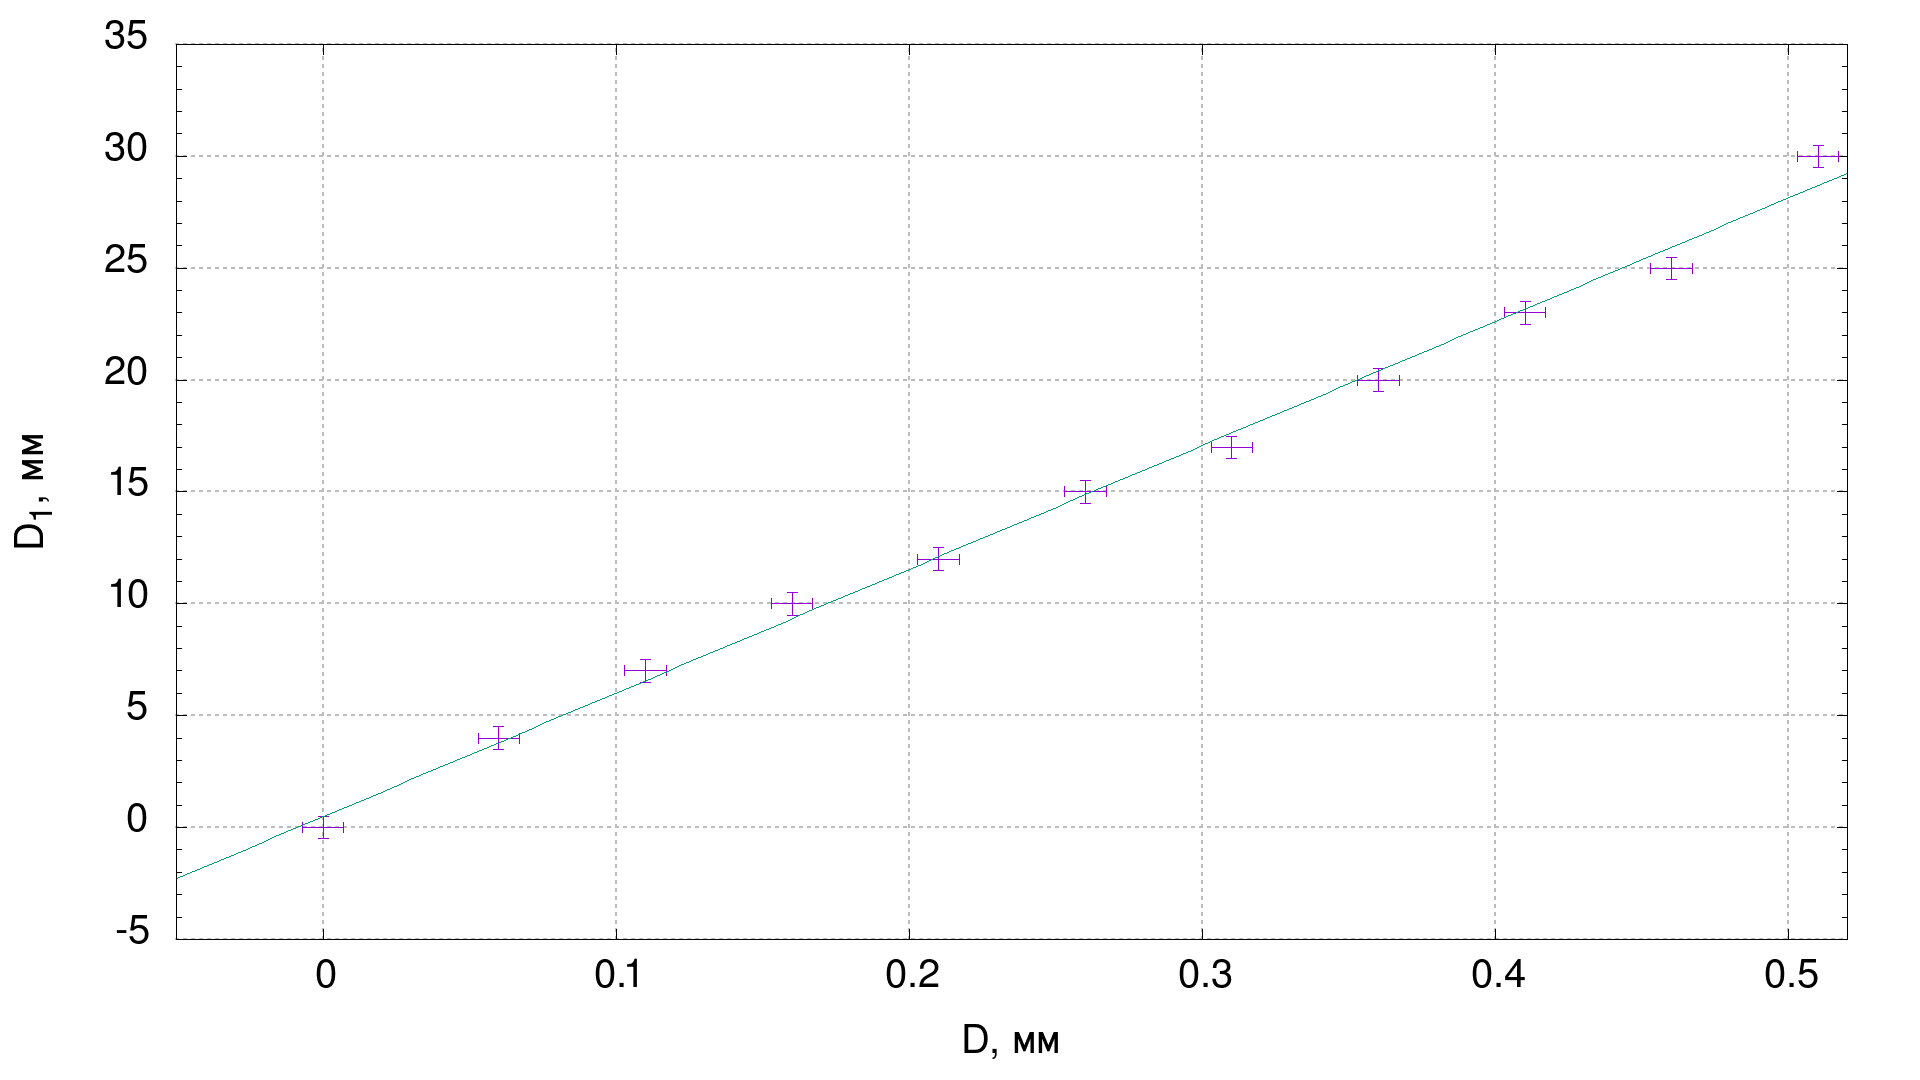
\includegraphics[width=0.95\textwidth]{plot1.png}
\end{center}

Из графика получим увеличение системы
\[\Gamma = 55\pm2.\]

\subsection*{6}
Далее посмотрим на значения значения $b_1=(1308\pm8)\,\text{мм}$ и $a_1 = \frac{Fb}{b-F} = (25.5\pm0.3) \text{мм}$ Получим, что увеличение
\[\Gamma = \frac{b}{a} = 51.3\pm0.9.\]
Это значение примерно совпадает с полученным ранее.

\section*{Определение ширины щели по ее спектру}
\subsection*{8-10}
Уберем линзу. Получим на удаленном экране спектр щели. Меняя ширину щели, проследим за изменением спектра на экране.

\begin{center}
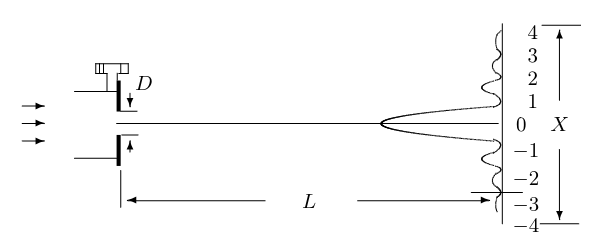
\includegraphics[width=0.95\textwidth]{2.png}
\end{center}

Для различных значений $D$, измерим расстояние $X_m$ между $m$ минимумами. Зная расстояние $L = (1332\pm8)\,\text{мм}$ от щели до экрана, получим значение ширины щели
\[D_\text{с} = \frac{\lambda L}{X_m/(m+1)},\]
где $\lambda = 532\,\text{нм}.$

\begin{center}
\begin{tabular}{|c|c|c|c|c|c|}\hline
$D_{\text{raw}}\text{, мкм}$&$D\text{, мкм}$&$m$&$X_m\text{, mm}$&$D_\text{с}\text{, мкм}$&$\Delta D_\text{с}\text{, мкм}$\\\hline
$160$&$20$&$3.0$&$90.0$&$31.49$&$0.17$\\\hline
$200$&$60$&$7.0$&$80.0$&$70.9$&$0.4$\\\hline
$250$&$110$&$13.0$&$82.0$&$121.0$&$0.7$\\\hline
$300$&$160$&$13.0$&$60.0$&$165.3$&$1.4$\\\hline
$350$&$210$&$17.0$&$60.0$&$212.6$&$1.8$\\\hline
$400$&$260$&$17.0$&$50.0$&$255$&$3$\\\hline
$450$&$310$&$15.0$&$37.0$&$306$&$4$\\\hline
$500$&$360$&$9.0$&$20.0$&$354$&$9$\\\hline
\end{tabular}\\~\\
$\Delta D_{\text{raw}}=5\,\text{мкм}, \Delta D=7\,\text{мкм}, \Delta X_m=0.5\,\text{mm}$
\end{center}



\begin{center}
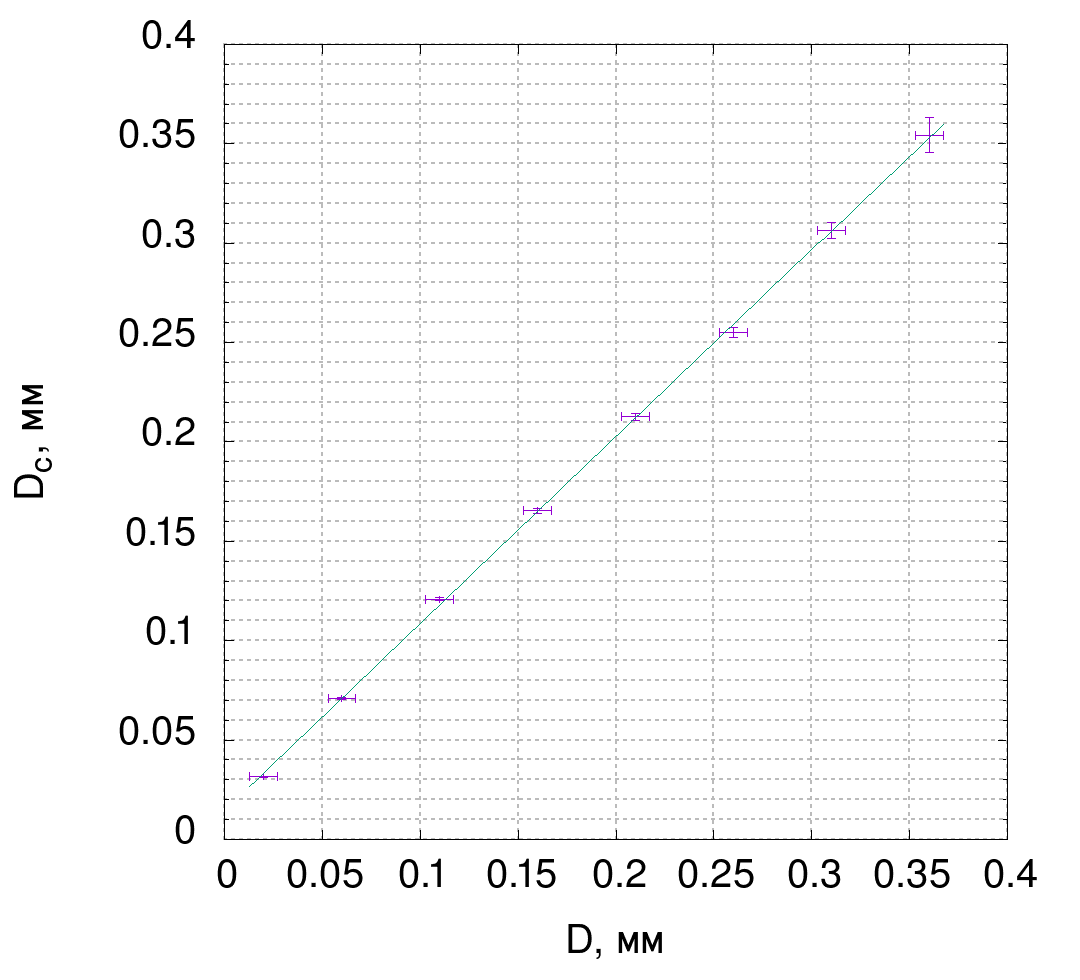
\includegraphics[width=0.95\textwidth]{plot2.png}
\end{center}

Из графика следует, что
\[\frac{D_c}{D} = 1.00\pm0.01\]


\section*{Определение периода по спектру на удаленном экране}
\subsection*{1-6}
Поставим кассету в двумерными решетками вплотную к выходному окну лазера и измерим расстояние $X_m$ между $m$ максимумами. Зная расстояние до экрана $L = (1300\pm8)\,\text{мм}$, получим период решетки
\[d = \frac{\lambda L}{X_m / m}.\]

\begin{center}
\begin{tabular}{|c|c|c|c|c|c|c|}\hline
$\text{\#решетки}$&$m$&$X_m\text{, мм}$&$X\text{, мм}$&$\Delta X\text{, мм}$&$d\text{, мкм}$&$\Delta d\text{, мкм}$\\\hline
$1$&$5.0$&$175.0$&$35.0$&$0.1$&$19.76$&$0.06$\\\hline
$2$&$7.0$&$165.0$&$23.57$&$0.07$&$29.34$&$0.09$\\\hline
$3$&$16.0$&$185.0$&$11.56$&$0.03$&$59.81$&$0.16$\\\hline
$4$&$31.0$&$185.0$&$5.968$&$0.016$&$115.9$&$0.3$\\\hline
$5$&$43.0$&$183.0$&$4.256$&$0.012$&$162.5$&$0.4$\\\hline
\end{tabular}\\~\\
$\Delta X_m=0.5\,\text{мм}$
\end{center}

\section*{Мультиплицирование}
\subsection*{1-2}
Поставим обратно тубус с щелью к окну лазера. Найдем на экране резкое щели с помозью линзы Л2. Подберем такое значение ширины щели, чтобы на экране можно было наблюдать мультиплицированное изображение сеток.

\begin{center}
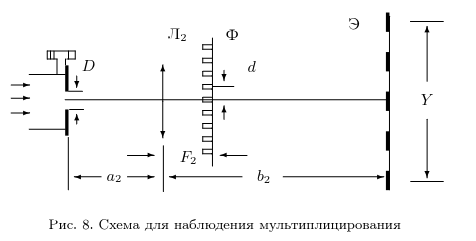
\includegraphics[width=0.95\textwidth]{3.png}
\end{center}

\subsection*{3-4}
Получим зависимость расстояния $Y$ между $K$ изображениями щели от номера решетки.

\begin{center}
\begin{tabular}{|c|c|c|c|c|c|c|}\hline
$\text{\#решетки}$&$Y\text{, мм}$&$K$&$K/Y\text{, 1/мм}$&$\Delta K/Y\text{, 1/мм}$&$d\text{, мкм}$&$\Delta d\text{, мкм}$\\\hline
$2.0$&$80.0$&$7.0$&$0.088$&$0.006$&$29.34$&$0.09$\\\hline
$3.0$&$40.0$&$7.0$&$0.175$&$0.013$&$59.81$&$0.16$\\\hline
$4.0$&$20.0$&$6.0$&$0.30$&$0.03$&$115.9$&$0.3$\\\hline
$5.0$&$15.0$&$7.0$&$0.47$&$0.03$&$162.5$&$0.4$\\\hline
\end{tabular}\\~\\
$\Delta Y=0.5\,\text{мм}$
\end{center}

Проверим линейность зависимости $K/Y$ от размера решетки.

\begin{center}
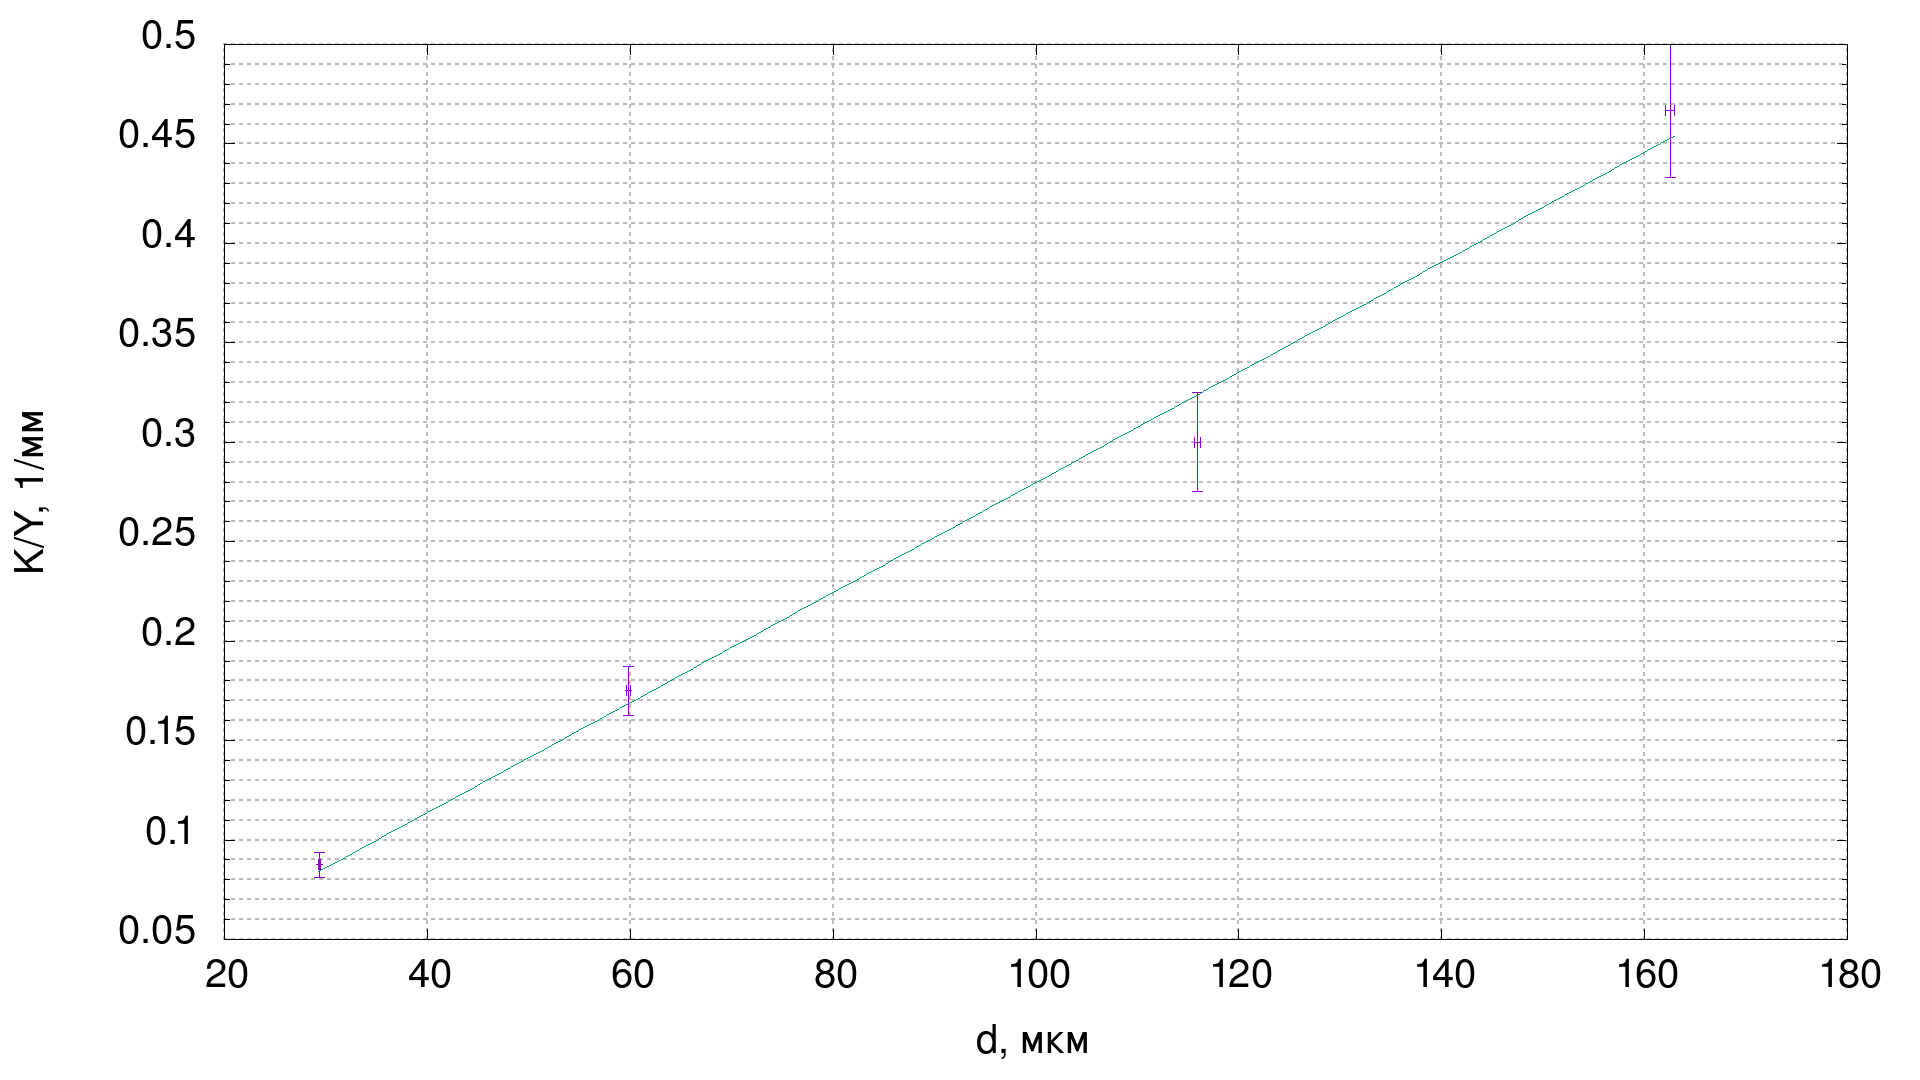
\includegraphics[width=0.95\textwidth]{plot3.png}
\end{center}

Как видно, зависимость линейная. Это подтверждает полученные в прошлом пункте результаты.

\section*{Вывод}
Мы научились исследовать параметры паттернов через порождающие дифракционные картины с помощью разложения в ряд фурье. В частности мы происследовали поведение щели и двумерных решеток. В экспериментах мы получили различные числовые значения, подтверждающие друг друга.

\end{document}








\lipsum[1-4]
\begin{wrapfigure}{R}{5cm}
\centering
\includegraphics[width=0.20\textwidth]{rd.png}
\caption{1}
\end{wrapfigure}
\lipsum[1-6]


\begin{figure}[h]
\begin{center}$
\begin{array}{cccc}
\includegraphics[width=0.20\textwidth]{rd.png}&
\includegraphics[width=0.20\textwidth]{rd.png}&
\includegraphics[width=0.20\textwidth]{rd.png}&
\includegraphics[width=0.20\textwidth]{rd.png}\\
(1) & (2) & (3) & (4)
\end{array}$
\end{center}
\end{figure}
